%%
% Please see https://bitbucket.org/rivanvx/beamer/wiki/Home for obtaining beamer.
%%
\documentclass[handout]{ctexbeamer}
% \mode<presentation> % change it to presentation model, but it does not work with [handout] option
\setCJKsansfont{SimSun}
\usepackage[T1]{fontenc}
\usepackage[utf8]{inputenc}
\usepackage{amssymb}
\usepackage{graphicx}
\usepackage{etoolbox} % adjust the space before and after figure
\usepackage{hyperref}
\usepackage{courier} % font for code in text
\usepackage{xeCJK} % Chinese 
\usepackage{listings}
\usepackage{wasysym}
\usepackage{amsthm} % for theorem definition style
\usepackage{rotating} % for the horizontal page table
\usepackage{pgfplots} % plot functions 
\usepackage{CJKutf8}
\usepackage{times}  

% \usepackage{enumitem} % never use this package for beamer
%\usepackage{theorem}  % define new environment, don't use this one for beamer  
\usepackage{url}
\usepackage{natbib}
\usepackage{bm} % bold math symbol
\usepackage{blkarray}  % for labeling row and columns of matrix
\usepackage{tikz}
\usetikzlibrary{calc}
\usetikzlibrary{matrix}
\usetikzlibrary{positioning}
\usepackage{color}
\usepackage{setspace}
\usepackage{bm} % bold math symbol
\usepackage{bibentry}
\nobibliography*
\usepackage{listings}
\usepackage[export]{adjustbox}
\usepackage[ruled,vlined]{algorithm2e}  % algorithm 

\setbeamertemplate{caption}[numbered]  % set the figure number
\usepackage{bbm} % indicator function

% select the theme and color
\usetheme{Boadilla}
\usecolortheme{beaver}

\lstset{language=Python}
\definecolor{mygreen}{rgb}{0,0.6,0}
\definecolor{mygray}{rgb}{0.5,0.5,0.5}
\definecolor{mymauve}{rgb}{0.58,0,0.82}
\lstset{
  backgroundcolor=\color{white},   % choose the background color; you must add \usepackage{color} or \usepackage{xcolor}; should come as last argument
  basicstyle=\footnotesize,        % the size of the fonts that are used for the code
  breakatwhitespace=false,         % sets if automatic breaks should only happen at whitespace
  breaklines=true,                 % sets automatic line breaking
  captionpos=b,                    % sets the caption-position to bottom
  commentstyle=\color{mygreen},    % comment style
  deletekeywords={...},            % if you want to delete keywords from the given language
  escapeinside={\%*}{*)},          % if you want to add LaTeX within your code
  extendedchars=true,              % lets you use non-ASCII characters; for 8-bits encodings only, does not work with UTF-8
  frame=single,	                   % adds a frame around the code
  keepspaces=true,                 % keeps spaces in text, useful for keeping indentation of code (possibly needs columns=flexible)
  keywordstyle=\color{blue},       % keyword style
  language=Matlab,                 % the language of the code
  morekeywords={*,...},            % if you want to add more keywords to the set
  numbers=left,                    % where to put the line-numbers; possible values are (none, left, right)
  numbersep=5pt,                   % how far the line-numbers are from the code
  numberstyle=\tiny\color{mygray}, % the style that is used for the line-numbers
  rulecolor=\color{black},         % if not set, the frame-color may be changed on line-breaks within not-black text (e.g. comments (green here))
  showspaces=false,                % show spaces everywhere adding particular underscores; it overrides 'showstringspaces'
  showstringspaces=false,          % underline spaces within strings only
  showtabs=false,                  % show tabs within strings adding particular underscores
  stepnumber=2,                    % the step between two line-numbers. If it's 1, each line will be numbered
  stringstyle=\color{mymauve},     % string literal style
  tabsize=2,	                   % sets default tabsize to 2 spaces
  title=\lstname,                  % show the filename of files included with \lstinputlisting; also try caption instead of title
  belowcaptionskip= 1 ex,
  belowskip = 1 ex
}


\title[]{察异辨花:简单得线性和非线性分类}
\subtitle{Introduction to linear and nonlinear methods for classification}

\date{\today}

\author[王斐]{王斐, Michael}
\institute[SenseTime, Edu]{SenseTime Edu, wangfei1@sensetime.com \and Math, Economics, Philosophy (UCD, Nottingham, CUHK) \and \url{https://github.com/Michael-yunfei/MDLforBeginners} \and 讲义、PPT、代码、图片设计}

%[January 2019] (optional)
%{Demo for SenseTime}

\usecolortheme[RGB={128,0,0}]{structure}

\newcommand{\zn}{\mathbb{Z}}
\newcommand{\cn}{\mathbb{C}}
\newcommand{\qn}{\mathbb{Q}}
\newcommand{\rn}{\mathbb{R}}
\newcommand{\pn}{\mathbb{P}}
\newcommand{\fn}{\mathbb{F}}
\newcommand{\nn}{\mathbb{N}}




\begin{document}
\definecolor{franceblue}{RGB}{14, 76, 96}
\definecolor{brightred}{RGB}{243, 66, 53}

%\setbeamercolor{block title alerted}{use=structure,fg=white,bg=structure.fg!75!black}
%\setbeamercolor{block body alerted}{parent=normal text,use=block title,bg=block title.bg!10!bg}

%\setbeamercovered{dynamic}  

\begin{frame}[noframenumbering]
  \titlepage
\end{frame}



\begin{frame}{本节内容}
	\tableofcontents
\end{frame}

\section{课程结构和进程简介}

\begin{frame}{课程结构}
第二章是我们高中教材机器学习的入门章节,本章可以说是整本教材最重要的章节,原因有:
\begin{itemize}
\setlength\itemsep{1em}
	\item 第一次开始介绍机器学习的数理模型
	\item 第一次系统介绍分类(人工智能领域70\%的问题是涉及分类)
	\item 透过本章了解机器学习的整个思路和流程
\end{itemize}

\hfil

辅导讲义的组成部分:
\begin{itemize}
\setlength\itemsep{1em}
	\item 课前预习C1 
	\item 课堂讲义C2 (讲义偏重数学严谨度,课堂偏重理解)
	\item 课后练习C3 (包括实验)
\end{itemize}

\hfil 

认真完成以上三个内容可以得到A, 只完成C1-C2可以得B。
\end{frame}

\begin{frame}{相关考核}
	考核机制的设计如下:
	
	\hfil
	
	\begin{itemize}
	\setlength\itemsep{1em}
		\item 课后练习C3 - 10\% 
		\item 期中考试 - 20 \% 
		\item 期末考试 - 30 \%
		\item 案例报告 - 40 \% (会讲故事+编程且调用相关程序)
	\end{itemize}
	
	\hfil 
	
	具体的考试形式和报告内容要求,后面会有具体的指示。
\end{frame}

\begin{frame}{课程结构和进程}
	写给辅导老师们的前言: 我们整个高中教材大体可以分为三大块:
	\begin{itemize}
	\setlength\itemsep{1em}
		\item 图片(分类,识别和聚类): Convolutional Neural Network
		\item 语音(识别,分类): Sequence Model (Recurrent NN)
		\item 文本(特征提取和分析): Sequence Model (RNN)
	\end{itemize}
	
	三个方向都涉及到深度学习模型(神经网络模型), 给学生介绍的时候,重点放在:
	
	\hfil
	\begin{itemize}
	\setlength\itemsep{1em}
		\item \underline{想象力}的构建上(后面我会在神经网络模型中介绍,很多巧妙的设计数学概念并不复杂,更多是需要想象力)
		\item 强化学生的\underline{人工智能思维}
		\item 强化学生的\underline{数据感觉和数据处理能力}
	\end{itemize}
\end{frame}

\begin{frame}{课程结构和进程}
由于神经网络模型背后的数学框架较为复杂,深入得讲解并不符合高中的教学目标,所以:

\hfill
\begin{itemize}
	\item 线性(感知器 perceptron)和非线性(支持向量机 support vector machines)分类就成为整个高中的教学重点 \begin{itemize}
	\item 数学模型要讲透彻: 理解每一个环节的公式和算法原理
	\item 机器学习框架下的编程要逐步解释: 学生必须可以自主完成感知器的算法编写
	\item 有条件得可以引导进行支持向量机的算法编写
	\item 课时安排: (1 + 2 + 6 = 9), 如果课堂讲解是3个小时,总课时就需要27个小时。(\underline{12个小时是必须的})
	\end{itemize}
	\item 对于神经网络模型的讲解: \begin{itemize}
	\item 可视化分析+案例演示
	\item 课外体验+参观 (很多模型训练时间长,需要算力大)
	\end{itemize}
\end{itemize}	
\end{frame}

\begin{frame}{第二章的重要性}
	我要在反复强调下第二章的重要性,你如果可以很好得理解第二章的模型,其它得才好举一反三,而且有助于我们学习神经网络模型。
	
	\hfil
	
	\begin{itemize}
	\setlength\itemsep{1em}
		\item 数学不好,没问题,不要担心;
		\item 会算加减乘除就可以学懂,要对自己有信心;
		\item 当然最重要的是要有耐心!(听课+练习+实验=12个小时)
	\end{itemize}
\end{frame}

\begin{frame}{课前预习题目浅析}
	课前预习第一部分是生活案例题,从生活中找一个分类的例子,然后描述下你是如何分类的(不超过60字),描述必须包含下面三个部分:
	
	\hfil
	
\begin{itemize}
\setlength\itemsep{1em}
	\item 分类的主体对象是什么?(比如,汽车,花草,等等)
	\item 分类的依据和标准是什么?
	\item 分类后如何衡量分类得好坏?
\end{itemize}
\end{frame}

\begin{frame}[fragile]{课前预习题目浅析}
分类简单讲就是: 寻找差异 (看起来不一样) 比如下面这种图,
\begin{figure}[H]
	\centering
	\includegraphics[width=0.6\textwidth]{fig/clothes}
\end{figure}
\end{frame}

\begin{frame}{课前预习作文题目浅析}
	因为事物的属性可以是很繁杂的,比如自然界中光是树木的科目分类就达到几万种(如果考虑不同植被的话,这个科目的量级会进一步上升, 吴征镒)。所以我们在对这些属性进行界定时,最简单有效的方式就是对其数字化(或者说有数字去测量和统计),比如下面这个案例。
	
	\begin{columns}
	\begin{column}{0.7\textwidth}
		\begin{table}[H]
		\centering
		\begin{tabular}{lccc}
		\hline 
			属种 & 代码 &花瓣长度 & 花瓣宽度 \\
			\hline 
			山鸢尾 & s1 & 1.4 & 0.2 \\
			山鸢尾 & s2 & 1.7 & 0.4 \\
			变色鸢尾 & ve1 & 3.9  & 1.4 \\
			变色鸢尾 & ve2& 4.9 & 1.5 \\
			维吉尼亚鸢尾 & vig1 & 6.9 & 2.3  \\
			维吉尼亚鸢尾 & vig2 & 6.1 & 1.9 \\
			\hline  
		\end{tabular}
\end{table}
	\end{column}
	\begin{column}{0.3\textwidth}
	\begin{figure}[H]
		\centering
		\includegraphics[width=0.9\textwidth]{fig/iris}
	\end{figure}	
	\end{column}
\end{columns}
\end{frame}

\section{数据阵(Dataframe)简介}

\begin{frame}[fragile]{数据阵定义}
	因为我们在机器学习领域经常接触数据阵,所以我们先来熟悉一下数据阵的概念和相关术语。
		
\begin{block}{定义}
	我们把由数字和对其的描述(有其根据)组成的信息形态,称为\textit{数据};我们将统一在一个样本下的数列,称为\text{数据组}(数据串); 有多个数据组构成的一系列数据,称为\textit{数据阵}。
\end{block}
\begin{figure}[H]
	\centering
	\includegraphics[width=0.67\textwidth]{/Users/Michael/Documents/MDLforBeginners/Notes/fig/dataframeEx.png}
\end{figure}

\underline{数 和 数据 的差别还是很大的!}
\end{frame}


\begin{frame}{数据阵的常用术语}
	因为我们几乎任何一个模型最初的切入点都是数据阵,所以很有必要统一下专业术语。
	\begin{figure}[H]
		\centering
		\includegraphics[width=0.96\textwidth]{fig/dataframeVis}
	\end{figure}
\end{frame}

\section{两个大脑论和人工智能的思维方式}

\begin{frame}{人工智能思维方式}
	这里我想给大家做一下思维转换,面向未来:
	\begin{itemize}
		\item 传统解决问题方案: 观察世界,抽象问题,解决问题
		\item 人工智能解决问题方案: 电脑观察世界,人抽象问题,两个大脑共同解决问题。
	\end{itemize}
	\begin{figure}[H]
		\centering
		\includegraphics[width=0.5\textwidth]{fig/C1MLbigpct}
	\end{figure}
	假定自然界运行有规律的话,那么对这些规律事件的记录和存储全部交给计算机,然后再由机器学习、深度学习模型\underline{对这些规律进行提取},从而进行预测。
\end{frame}

\begin{frame}{人工智能思维方式}
现在我们就通过\underline{分类问题}来理解人工智能的思维方式!
\begin{figure}[H]
	\centering
	\includegraphics[width=0.9\textwidth]{fig/C2preIris}
	\caption{鸢尾花数据阵的可视化}
\end{figure}	
注意: 二维图表中只能构图\underline{两个属性}
\end{frame}


\section{分类和线性分类}

\begin{frame}{什么是分类?}
	\begin{block}{定义}
	分类指的是根据事物不同的属性,对某个或一些物体进行划分的过程。在没有任何属性的情况下,我们不能进行分类。在有属性的情况下,我们可以依据属性,进行分类,比如黑猫和白猫。
\end{block}

从哲学的角度上讲,存在的便是有属性的在。绝对的存在(即无属性的纯存在)在中文哲学的概念里指的是`道’(老子里有一句名言: 道生一,一生二,三生万物),在西方哲学里指的是`上帝'。黑格尔有一句名言:绝对得有即是绝对得无(纯有等同于纯无,中文:白马非马)
\begin{itemize}
	\item 人 - 属性: 男女,身高,体重,肤色...
	\item 花 - 属性: 颜色,开花季节...
	\item 书本 - 重量,颜色,科目
\end{itemize}
\end{frame}

\begin{frame}{什么是线性分类}
	\begin{example}
		在预习题目中,我们要求同学们求解下列的方程组:
	\begin{align*}
	& 56w_1 + 8 w_2 = 36 \\
	& 32 w_1+ 4 w_2 + w_3 = 20.5 \\
	& 48 w_1 + 3w_2 + w_3 = 29.8 \\
	& \begin{bmatrix}
		56 & 8 & 0 \\
		32 & 4 & 1 \\
		48 & 3 & 1 
	\end{bmatrix} \begin{bmatrix}
		w_1 \\
		w_2 \\
		w_3
	\end{bmatrix} = \begin{bmatrix}
		36 \\
		20.5 \\
		29.8 
	\end{bmatrix} 
\end{align*}
稍加计算便可以得出:
\begin{align*}
	w_1= 0.6; \ \ \ w_2 = 0.3; \ \ \ w_3 = 0.1 
\end{align*}
	\end{example}
	这个题目是老师专门设计过的,其背后的场景为下面的表格。
\end{frame}

\begin{frame}{什么是线性分类}
	\begin{figure}[H]
		\centering
		\includegraphics[width=0.9\textwidth]{fig/C1C2grade}
	\end{figure}
	\begin{example}
	\begin{align*}
		X \cdot w & = Y \\
		\begin{bmatrix}
		56 & 8 & 0 \\
		32 & 4 & 1 \\
		48 & 3 & 1 
	\end{bmatrix} \begin{bmatrix}
		w_1 \\
		w_2 \\
		w_3
	\end{bmatrix} & = \begin{bmatrix}
		36 \\
		20.5 \\
		29.8 
	\end{bmatrix}
	\end{align*}	
	\end{example}
\end{frame}

\begin{frame}{什么是线性分类}
	如果假定学习的各种属性(学习时间、练习题目数量,等)与结果(成绩)存在简单的线性关系的话,解方程可以告诉我们:
\begin{itemize}
	\item $w_1 = 0.6$, 即学习时间对成绩的影响比重约为60\%;
	\item $w_2 = 0.3$, 即练习题目的数量对成绩的影响比重约30\%;
	\item $w_3 = 0.1$, 即考前睡眠对成绩的影响比重约10\%。
\end{itemize}

虽然这个题目很简单的,但是其反应了机器学习的一般框架:
\begin{itemize}
	\item 假定自然界中的事物发展是有规律的
	\item 这些规律被记录存储为数字和文本形式($X, Y$)
	\item 人类根据对问题的抽象设定相关的框架和模型(例如,线性方程)
	\item 结合模型和数据,获得规律参数$w$
	\item 拿到规律参数$w$后,再去预测
\end{itemize}
\end{frame}

\begin{frame}{什么是线性分类}
现在我们从鸢尾花数据阵中随意取三个样本,然后属性也取三个$X= 3 \times 3, Y = 3 \times 1$, 然后解方程
\begin{table}[H]
		\centering
{\footnotesize
		\begin{tabular}{lcccc}
		\hline 
			属种 & 代码 & 花萼宽度(a=1.1) &花瓣长度(b=-3.7) & 花瓣宽度(c=9.) \\
			\hline 
			山鸢尾 & 0 & 3 &  1.4 & 0.2 \\
			变色鸢尾 & 1 & 3.2 & 4.5  & 1.5 \\
			维吉尼亚鸢尾 & 2 & 2.7 &  5.1 & 1.9  \\
			\hline  
		\end{tabular}
}
\end{table}
我们可以理解大自然在不同的鸢尾花进化时,特意的分配了下面的规律参数:
		\begin{itemize}
			\item 花萼宽度(1.1)
			\item 花瓣长度(-3.7)
			\item 花瓣宽度(9.4)
		\end{itemize}
	\underline{沿用这种进行线性分类存在一个很大的问题}
\end{frame}

\begin{frame}{从线性回归引入到分类}
再看一下表格
		\begin{table}[H]
		\centering
		\begin{tabular}{lccc}
		\hline 
			属种 & 结果($y$) &花瓣长度 & 花瓣宽度 \\
			\hline 
			山鸢尾 & 0 & 1.4 & 0.2 \\
			山鸢尾 & 0 & 1.7 & 0.4 \\
			变色鸢尾 & 1 & 3.9  & 1.4 \\
			变色鸢尾 & 1& 4.9 & 1.5 \\
			维吉尼亚鸢尾 & 2 & 6.9 & 2.3  \\
			维吉尼亚鸢尾 & 2 & 6.1 & 1.9 \\
			\hline  
		\end{tabular}
\end{table}	
\end{frame}

\begin{frame}{从线性回归引入到分类}
\begin{figure}[H]
	\centering
	\includegraphics[width=0.9\textwidth]{fig/logisticreg1}
\end{figure}	
\end{frame}


\begin{frame}{从线性回归引入到分类}
\begin{figure}[H]
	\centering
	\includegraphics[width=0.9\textwidth]{fig/logisticreg2}
\end{figure}	
\end{frame}

\begin{frame}{从线性回归引入到分类}
引入逻辑回归(logistic regression), sigmoid function:
	\begin{align*}
		\sigma(z) = \frac{1}{1+e^{-z}} = \frac{1}{1+e^{X\beta + \varepsilon}}
	\end{align*}
	\begin{figure}[H]
		\centering
		\includegraphics[width=0.9\textwidth]{fig/logisticreg3}
	\end{figure}
\end{frame}



\begin{frame}{线性分类的切入}
	线性分类的切入:
	\begin{itemize}
	\setlength\itemsep{0.6em}
		\item 延续线性回归思路,需要转换$Y$轴,借助logistic regression(sigmoid function) 
		\item 不延续线性回顾思路,完全代数性质(点积)
	\end{itemize}
	\begin{align*}
		a \cdot b = ||a|| ||b|| \cos \theta
	\end{align*}
	\begin{figure}[H]
		\centering
		\includegraphics[width=0.5\textwidth]{fig/C2C2svmprojc}
	\end{figure}
\end{frame}

\begin{frame}{线性分类的切入}
	\begin{align*}
		a \cdot b & = ||a|| ||b|| \cos \theta \\
		&= ||a|| ||b|| \cos \theta  \begin{cases}
		> 0 &  0 \leq \theta < \frac{\pi}{2} \\
		= 0 & \theta = \frac{\pi}{2}  \ \ \text{即$a$与$b$垂直} \\
		< 0 &  \frac{\pi}{2} < \theta \leq \pi 
	\end{cases}
	\end{align*}
	\begin{figure}[H]
		\centering
		\includegraphics[width=0.5\textwidth]{fig/C2C2svmprojc}
	\end{figure}
\end{frame}

\begin{frame}{线性分类的切入}
Vladimir Vapnik 还活着,所以可以了解到最初他是如何创立支持向量机(Support vector machine)的。
\begin{columns}
\begin{column}{0.3\textwidth}
\centering
\includegraphics[width=\textwidth]{fig/P2dotpTable}
\end{column}
\begin{column}{0.7\textwidth}
	\begin{figure}[H]
	\centering
	\includegraphics[width=\textwidth]{fig/C2C2dotprodt}
\end{figure}	
\end{column}
\end{columns}
Reference: Patrick Winston (Youtube, 点击率1百万)
\end{frame}

\begin{frame}{什么是线性分类}
	\begin{block}{定义}
	我们把可以表现为下列形式的方程,称为\textit{线性方程}:
	\begin{align*}
		a_1 x_1 + a_2 x_2 + \cdots + a_n x_n + b = 0
	\end{align*}
	其中$x_1, x_2, \cdots, x_n$ 为变量, $a_1, a_2, \cdots, a_n$ 为系数。
\end{block}
线性方程本质是一种累计的过程,因为乘法也是加法,比如$3 \times 5 = 5 + 5 + 5 = 15$。我们刚才计算的那几个例子都是线性的。
\end{frame}

\begin{frame}{什么是线性分类}
	\begin{example}
现实生活中,有些关系可以表现为线性关系,有些关系不可以表现为线性关系,比如,
\begin{align*}
	a_1 x_1^2 + a_2 \sin (x_2) + a_3 e^{x_3} + b  = 0 
\end{align*}	
当$x_1, x_2, x_3$之间的关系为非线性是,我们可以对其进行线性转换,比如:
\begin{align*}
	x'_1 = x_1^2; \ \ \ x'_2 = \sin (x_2); \ \ \ x'_3 = e^{x_3}
\end{align*}
那么新的关系就变成了线性: 
\begin{align*}
	a_1 x'_1 + a_2 x'_2 + a_3 x'_3 = 0 
\end{align*}
\end{example}
\end{frame}

\begin{frame}{什么是线性分类}
\begin{figure}[H]
	\centering
	\includegraphics[width=0.7\textwidth]{fig/C2C2linear}
\end{figure}	
\end{frame}

\begin{frame}{什么是线性分类:矩阵和向量点积}
\begin{definition}
	\textit{矩阵}(Matrix)是一个按照长方阵列排列的复数或实数集合。对一个矩阵的简单描述可以为 $m \times n$ 的矩阵,即该矩阵有$m$ 行,$n$列. $m \times n$也被称为矩阵的大小。
\end{definition}

\begin{example}
比如,我们有$3 \times 3 $的矩阵$A$ 和$2 \times 3$ 的矩阵$B$。
\begin{align*}
	 A = \begin{bmatrix}
	1 & 3 & 4 \\
	2 & 5 & 8 \\
	3 & 9 & 7
\end{bmatrix}, & & B = \begin{bmatrix}
	3.2 & 1.9 & 5.7 \\
	4.1 & 5.8 & 9.3 \\
\end{bmatrix}
\end{align*}	
\end{example}
\end{frame}

\begin{frame}{什么是线性分类:矩阵和向量点积}
\begin{definition}
	矩阵中单独的一行被成为\textit{行向量}(row vector), 单独的一列别成为\textit{列向量}(column vector)。
\end{definition}
\begin{example}
比如在上面的矩阵$A$中,	我们有以下单独的向量:
\begin{align*}
 & A = \begin{bmatrix}
	1 & 3 & 4 \\
	2 & 5 & 8 \\
	3 & 9 & 7
\end{bmatrix} \\
	& A_{r2} = [2 \ 5 \ 8],   & A_{c2} = \begin{bmatrix}
		3 \\
		5 \\
		9 
	\end{bmatrix}
\end{align*}
\end{example}
\end{frame}

\begin{frame}{什么是线性分类:向量点积}
矩阵和向量的运算,是根植于方程中变量与系数(规律参数)的对应关系来的。我们这一小节中重点学习向量运算,下一章中开始学习矩阵运算。比如,下面的方程可以转为向量相乘:
		\begin{align*}
			2a + 3b + c = 3 \ \ \Leftrightarrow \ \ \begin{bmatrix}
				2 & 3 & 1
			\end{bmatrix} \begin{bmatrix}
				a \\
				b \\
				c
			\end{bmatrix} = [3] 
		\end{align*}
		因为变量和系数,必须相对应,所以下面的运算一个是不合法的,另外两个是不合法的:
		\begin{align*}
			\begin{bmatrix}
				2 & 3 & 0
			\end{bmatrix} \begin{bmatrix}
				a \\
				b 
			\end{bmatrix} & & \begin{bmatrix}
				2 & 3 & 1
			\end{bmatrix} \begin{bmatrix}
				a \\
				b \\
				c
			\end{bmatrix} & & \begin{bmatrix}
				2 & 3 & 1
			\end{bmatrix} \begin{bmatrix}
				a \\
				b 
			\end{bmatrix}
		\end{align*}	
		点积运算时,\underline{向量维数}必须相同:同位元素相乘后累加。(不要说向量的长度,长度是另外的概念)
\end{frame}

\begin{frame}{什么是线性分类:向量点积}
\begin{definition}
	已知两个维数相同的向量$w=[w_1, w_2, \cdots, w_n]$ 和$X = [x_1, x_2, \cdots, x_n]$, 那么向量的相乘,也并被成为点积(dot product)定义为:
\begin{align*}
		 X \cdot a & = \begin{bmatrix}
		x_1 & x_2 & \cdots & x_n
	\end{bmatrix} \begin{bmatrix}
		w_1 \\
		w_2 \\
		\vdots \\
		w_n
	\end{bmatrix} \\
	 w \cdot X & = \begin{bmatrix}
		w_1 & w_2 & \cdots & w_n
	\end{bmatrix} \begin{bmatrix}
		x_1 \\
		x_2 \\
		\vdots \\
		x_n
	\end{bmatrix}\\
	& =  \sum_{i=1}^n x_i w_i = a_1 w_1 + a_2 w_2 + \cdots + a_n w_n 
\end{align*}
\end{definition}
\end{frame}

\begin{frame}{什么是线性分类:向量点积几何性质}
\begin{definition}
	当两个向量的点积运算结果为$0$时,我们称这两个向量\textit{正交},或者互为正交向量,数学表示为:
	\begin{align*}
		 X \cdot w = <X, w> = 0 \ \ \Leftrightarrow \ \ \sum_{i=1}^n  x_i w_i =  x_1 w_1 +  x_2 w_2 + \cdots +  x_n w_n = 0 
	\end{align*}
\end{definition}

两个向量正交时,在几何上表现为垂直(perpendicular),比如
\begin{align*}
	u \cdot v = \begin{bmatrix}
		2 & 1 
	\end{bmatrix} \begin{bmatrix}
		-1 \\
		2
	\end{bmatrix} = -2 + 2 = 0 & &  z \cdot x = \begin{bmatrix}
		0 & 0 & 1
	\end{bmatrix} \begin{bmatrix}
		1 \\
		0 \\
		0
	\end{bmatrix} = 0 
\end{align*}		
\end{frame}

\begin{frame}{什么是线性分类:向量点积几何性质}
两个向量正交时,在几何上表现为垂直(perpendicular),比如
\begin{figure}[H]
	\centering
		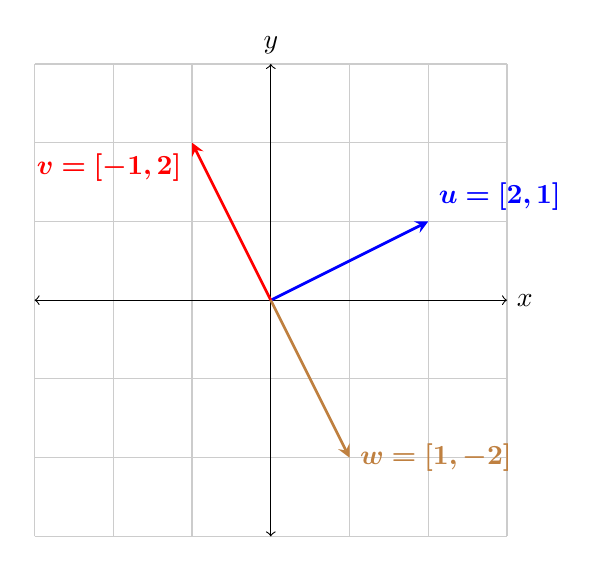
\begin{tikzpicture}
  \draw[thin,gray!40] (-3,-3) grid (3,3);
  \draw[<->] (-3,0)--(3,0) node[right]{$x$};
  \draw[<->] (0,-3)--(0,3) node[above]{$y$};
  \draw[line width=1pt,blue,-stealth](0,0)--(2,1) node[anchor=south west]{$\boldsymbol{u=[2, 1]}$};
  \draw[line width=1pt,red,-stealth](0,0)--(-1,2) node[anchor=north east]{$\boldsymbol{v=[-1, 2]}$};
  \draw[line width=1pt,brown, -stealth](0,0)--(1, -2) node[right]{$\boldsymbol{w=[1, -2]}$};
\end{tikzpicture}
\end{figure}
注意$w\cdot u=0$, 他们在几何上垂直,在代数上正交(orthogonal)。	
\end{frame}

\begin{frame}{什么是线性分类:向量点积几何性质}
整个感知器分类和支持向量机,完全可以用下面这张图来概括。
\begin{columns}
\begin{column}{0.3\textwidth}
\centering
\includegraphics[width=\textwidth]{fig/P2dotpTable}
\end{column}
\begin{column}{0.7\textwidth}
	\begin{figure}[H]
	\centering
	\includegraphics[width=\textwidth]{fig/C2C2dotprodt}
\end{figure}	
\end{column}
\end{columns}
\end{frame}

\begin{frame}{感知器线性分类(perceptron)}
	\begin{definition}
	假设自然界中可分类对象具有一定属性,且属性个数大于$1$,当其属性的特征变量($X$)与其属性的规律参数($w$)存在下列线性关系时:
	\begin{align*}
		X \cdot w + b  =0 ; \ \ \ \Leftrightarrow \ \ \ x_1 w_1 + x_2 w_2 + \cdots + x_n w_n + b = 0
	\end{align*}
	(其中$n$为分类对象的属性个数),我们将其称为\textit{可线性分类}。因为该公式的点积为零,所以我们将其转换为下列的格式:
	\begin{align*}
		\begin{bmatrix}
			X & 1
		\end{bmatrix} \begin{bmatrix}
			w \\
			b
		\end{bmatrix} = 0  
	\end{align*}
	其中$b$为常数变量(无属性变量), 我们将向量$w$和$x$组成的分界面以及正交矢量(在二维中,就是一条线和其垂直线)称为\textit{感知器}(percepton),其中$w$就是我们需要计算的规律参数,而$X$则是由我们采集的数据组成的特征变量
	\end{definition}
\end{frame}

\begin{frame}{感知器线性分类(perceptron)}
只能\underline{二分}! 但是自然界很多问题二分也足够了:
\begin{itemize}
	\item 黄猫 V.S. 非黄猫
	\item 蓝猫 V.S. 非蓝猫
	\item 重复二分等同于多类分法
\end{itemize}
\begin{columns}
\begin{column}{0.3\textwidth}
\centering
\includegraphics[width=\textwidth]{fig/P2dotpTable}
\end{column}
\begin{column}{0.7\textwidth}
	\begin{figure}[H]
	\centering
	\includegraphics[width=\textwidth]{fig/C2C2dotprodt}
\end{figure}	
\end{column}
\end{columns}
\end{frame}


\begin{frame}{感知器线性分类(perceptron)}
感知器被定义为:
\begin{align*}
	& X \cdot w + b  = 0 \\
	& x_1 w_1 + x_2 w_2 + \cdots + x_n w_n + b  =0
\end{align*}	
也就是下图中的蓝色和红色的向量。
\begin{figure}[H]
	\centering
	\includegraphics[width=0.8\textwidth]{fig/C2C2dotprodt}
\end{figure}	
\end{frame}

\begin{frame}{感知器线性分类(perceptron)过程}
	\begin{block}{感知器分类}
	我们将向量$w$和$x$组成的分界面以及正交矢量(在二维中,就是一条线和其垂直线)称为\textit{感知器}(percepton),其中$w$就是我们需要计算的规律参数,而$x$则是由我们采集的数据组成的特征变量。感知器分类一个\textbf{二分}过程,分类过程如下:
	\begin{align*}
		\hat{y} = \begin{cases}
			+1 & x \cdot w > 0 \\
			-1 & x \cdot w < 0
		\end{cases}
	\end{align*}
	其中$\hat{y}$是我们在进行分类是需要预测的结果。	
	\end{block}
\begin{table}[H]
	\centering
	\begin{tabular}{cccccc}
		\hline 
		样本 & 花瓣长度 & 花瓣宽度 & 统计结果 & 重新标注 & 预测结果 \\
		\hline 
		山鸢尾 & 2 & 1.6 & 0 & 1 & 1  \\
		变色鸢尾 & 1.3 & 0.7 & 1 & -1 & 1  \\
		维吉尼亚鸢尾 & 1.1 & 0.8 & 2 & -1 &  -1 \\
		\hline  
	\end{tabular}
\end{table}
\end{frame}

\begin{frame}{感知器线性分类(perceptron)过程}
	\begin{figure}[H]
		\centering
		\includegraphics[width=\textwidth]{fig/C2prevIris2}
		\caption{鸢尾花二分展示}
	\end{figure}
\end{frame}


\section{损失函数(Loss Function)}

\begin{frame}{损失函数}
拥有了标注的数据,就有了\underline{对比依据}\footnote[frame]{对,没有对比就没有伤害。}, 就可以训练人工智能模型,从而可以调整模型参数,来提升预测准确度。而用来衡量准确度的方程就需要损失方程。

\hfil

\begin{definition}
	假设数据阵标注过的数据准确可靠,在机器学习模型中,模型在根据学习到参数规律对特征变量(统计的数据)计算后输出的结果$\hat{Y}$与数据阵\footnote{(注意是`数据阵',所以是衡量的是模型在整个数据阵下的表现)}标注的数据结果$Y$差别的函数统称为\textit{损失函数(Loss Function)}。损失方程的一般形式为:
\begin{align*}
	L(Y, \hat{Y}): \ \to \rn 
\end{align*}	
\end{definition}
\end{frame}

\begin{frame}{感知器损失函数}
\begin{definition}
	给定机器学习模型,对单个数据串的预测准确度的衡量的方程,被成为测量公式(cost function),例如,$x_1$为一个数据串\footnote{即为$1 \times n$的向量,重复记忆$m \times n$, $m$样本数,$n$属性个数。},$w$是我们的训练得出的规律参数,$\hat{y}_1$为我们预测的结果,$y_1$为数据串标注的结果,那么我们的测量公式(cost function) 为:
	\begin{align*}
		y_1 - \hat{y}_1 = y_1 - x_1 \cdot w 
	\end{align*}
	实际上,损失函数(Loss function)就是对测量公式的求和:
	\begin{align*}
		L = \sum_{i=1}^m y_i - \hat{y}_i 
	\end{align*}
	其中$L$为损失函数。
\end{definition}
\end{frame}


\begin{frame}{感知器损失函数}
我们来详细解释下在感知分类中所定义的损失函数,以及为什么我们需要其最小化。再重复一下,$y_i$为标注的结果,$\hat{y}_i$为模型预测的结果,我们看一下具体的计算:
		\begin{align*}
				-(y_i \times \hat{y}_i) = \begin{cases}
					-1 & \text{如果$y_i = 1, \hat{y_i} = 1$, 预测正确} \\
					-1 & \text{如果$y_i = -1, \hat{y_i} = -1$, 预测正确} \\
					1 & \text{如果$y_i = 1, \hat{y}_i  -1$, 预测错误} \\
					1 & \text{如果$y_i = -1, \hat{y}_i = 1$,预测错误} 
				\end{cases}
		\end{align*}
	那么由此得出的测量方程(cost function)为:
		\begin{align*}
				c_i = \max \{ 0, -(y_i \times \hat{y}_i) \}  = \begin{cases}
					0 & \text{如果$y_i = 1, \hat{y_i} = 1$, 预测正确} \\
					0 & \text{如果$y_i = -1, \hat{y_i} = -1$, 预测正确} \\
					1 & \text{如果$y_i = 1, \hat{y}_i  -1$, 预测错误} \\
					1 & \text{如果$y_i = -1, \hat{y}_i = 1$,预测错误} 
				\end{cases}
		\end{align*}	
\end{frame}


\begin{frame}{感知器损失函数}
那么最终的损失函数为,
		\begin{align*}
			L = \sum_{i=1}^m c_i = \sum_{i=1}^m \max \{ 0, - (y_i \times \hat{y}_i) \} = \sum_{i=1}^m \mathbbm{1} [ \text{预测错误}] 
		\end{align*}
		因为损失函数统计的是预测错误的情况,所以我们希望最小化该损失函数,因为当预测错误的情况越少时,准确率越高,模型表现越好:
		\begin{align*}
			\min_{w}  L = \sum_{i=1}^m c_i & = \sum_{i=1}^m \max \{ 0, - (y_i \times \hat{y}_i) \} \\
			&  = \sum_{i=1}^m \mathbbm{1} [ \text{预测错误}]  \\
			& = \sum_{i=1}^m \max \{ 0, -y_i \times (x_i \cdot w) \}
		\end{align*}	
\end{frame}


\section{梯度下降法(Gradient Descent)}

\begin{frame}{理解梯度下降法(Gradient Descent)}
	一旦确定了我们的损失函数后,我们希望最小化我们的函数,这样损失越小,准确率越高:
	\begin{align*}
			\min_{w}  L = \sum_{i=1}^m c_i & = \sum_{i=1}^m \max \{ 0, - (y_i \times \hat{y}_i) \} \\
			&  = \sum_{i=1}^m \mathbbm{1} [ \text{预测错误}]  \\
			& = \sum_{i=1}^m \max \{ 0, -y_i \times (x_i \cdot w) \}
		\end{align*}	
\begin{itemize}
	\item 优化问题需要借助导数的概念
	\item 天不生仲尼(牛顿)亘古如长夜
\end{itemize}
\end{frame}

\begin{frame}{理解梯度下降法(Gradient Descent)}
	\begin{definition}
	设有定义域和取值在实数域中的函数$y=f(x)$。若$f(x)$在点$x_0$的某个邻域内有定义,则当自变量$x$在$x_0$处取得增量$\Delta x$时,$y$相应地取得增量$\Delta y = f(x_0 + \Delta x) - f(x_0)$;当$\Delta y$与$\Delta x$之比在$\Delta x \to 0$时极限存在,则称函数$y=f(x)$在点$x_0$处可导,并称这个函数在$x_0$点处的\textit{导数},记为$f'(x_0)$,即:
	\begin{align*}
		f'(x_0) = \lim_{\Delta x \to 0} \frac{\Delta y}{\Delta x} = \lim_{\Delta x \to 0} \frac{f(x_0 + \Delta x) - f(x_0)}{\Delta x}
	\end{align*}
\end{definition}
对以上定义,对于高中生来说,不需要太在意细节,我们需要重点了解其变化率的意涵。
\end{frame}

\begin{frame}{理解梯度下降法(Gradient Descent)}
我们还是通过下面的例子来理解导数变化率的概念:
\begin{align*}
	f(x) & = -x^2 + 2x + 3 \\
	f'(x) & = -2x + 2 \\
\end{align*}
\begin{figure}[H]
	\centering
	\includegraphics[width=0.8\textwidth]{fig/C2preGrades}
\end{figure}
\end{frame}

\begin{frame}{理解梯度下降法(Gradient Descent)}
\begin{figure}[H]
	\centering
	\includegraphics[width=0.6\textwidth]{fig/C2preGd2}
\end{figure}	
\end{frame}


\begin{frame}{理解梯度下降法(Gradient Descent)}
\begin{figure}[H]
	\centering
	\includegraphics[width=0.96\textwidth]{fig/C2C2GradientDes}
\end{figure}	
\end{frame}

\begin{frame}{梯度下降法(Gradient Descent)}
\begin{definition}
	选定初始值$\theta_0$, 梯度下降法(Gradient Descent)通过下面的公式去逐步计算$\theta_1, \theta_2, \cdots$,直到达到我们满意的结果(可以是计算的次数,也可以是计算的误差):
	\begin{align*}
		\theta_{t+1} = \theta_t - \alpha \nabla f(\theta_t)
	\end{align*}
	其中,$\alpha$是为更新参数(learning rate), $\nabla f(\theta_t)$为公式$f(\cdot)$在$\theta_t$时的导数值。因为在机器学习领域,$f(\cdot)$为我们所定义的损失函数(Loss function), 所以我们希望最小化损失,因此是
	\begin{align*}
		\theta_{t+1} = \theta_t - \alpha \nabla f(\theta_t)
	\end{align*}
	而不是
	\begin{align*}
		\theta_{t+1} = \theta_t + \alpha \nabla f(\theta_t)
	\end{align*}
\end{definition}
\end{frame}


\begin{frame}{梯度下降法(Gradient Descent)}
梯度下降法的一般公式为(因为多数情况下是求最小值): 
\begin{align*}
		\theta_{t+1} = \theta_t - \alpha \nabla f(\theta_t)
	\end{align*}
注意更新参数(learning rate) $\alpha$的选择对于我们找到期望的$\theta$值有比较大的影响。一般可概括为:
\begin{itemize}
	\item $\alpha$ 较小时, 需要多次计算,$\theta$的更新较慢;
	\item $\alpha$ 较大时,计算次数下降,但是每次更新可能会错过期望值。
\end{itemize}
具体到$\alpha$的选择时,我们后面在结合不同的案例时,还会进一步讲解。	
\end{frame}


\begin{frame}{感知器二元分类算法}
在理解了什么是损失函数和梯度下降法后,我们来学习感知器分类的具体算法。这个算法的核心要点为:
	\begin{itemize}
		\item 假设分类问题可线性分类,即符合下列分类过程 \begin{align*}
		\hat{y} = \begin{cases}
			+1 & x \cdot w + b > 0 \\
			-1 & x \cdot w  + b < 0
		\end{cases}
	\end{align*}
	其中$\hat{y}$为我们再分类过程中需要标注的结果,$x$为$1\times n$的向量,表示分类对象有$n$个属性,$w$长度为$1 \times n$,表示为分类属性的规律参数。注意我们如果把点积写成矩阵的相乘的话应该是$x w^T$。
	\item 我们设定的损失函数为 \begin{align*}
		L = \sum_{i=1}^m c_i = \sum_{i=1}^m \max \{ 0, - y_i \times (x_i \cdot w + b) \} 
	\end{align*}
	\end{itemize}
\end{frame}

\begin{frame}{感知器二元分类算法}
	\begin{itemize}
		\item  损失函数的导数为:$\frac{\partial L}{\partial w} = \{ 0, -y_i \times x_i \}$, 等同于
	\begin{align*}
		\frac{\partial L}{\partial w} & = - y_i \times x_i; \ \ \ \text{当$x_i \cdot w < 0$时} \\
		\frac{\partial L}{\partial w} & = 0; \ \ \ \ \ \ \ \ \ \ \text{当$x_i \cdot w > 0$时}
	\end{align*}
	\item 根据梯度下降法的公式(求最小值),我们对规律参数的更新公式为: \begin{align*}
		w_{t+1} & = w_{t} - \alpha \frac{\partial L}{\partial w} \\
		& = w_{t} + \alpha (y_i \times x_i) \tag{当$x_i \cdot w < 0$}
	\end{align*}
	\end{itemize}
\end{frame}


\begin{frame}{感知器二元分类算法}
教材中的公式,假设我们的数据阵中有两个属性和一个自变量$b$,那么我们的算法就变为: 
\begin{itemize}
	\item 假设分类问题可线性分类,即符合下列分类过程 \begin{align*}
		\hat{y} = \begin{cases}
			+1 & x^{[1]} a_1 + x^{[2]} a_2 + b > 0 \\
			-1 & x^{[1]} a_1 + x^{[2]} a_2 + b < 0
		\end{cases}
	\end{align*}
	\item 我们设定的损失函数为 \begin{align*}
		L = \sum_{i=1}^m c_i = \sum_{i=1}^m \max \{ 0, - y_i \times (x^{[1]}_i a_1 + x^{[2]}_i a_2 + b_i) \} 
	\end{align*}
	\item 损失函数的导数为:$\frac{\partial L}{\partial a_1} = \{ 0, -y_i \times x_i^{[1]} \}$, 等同于
	\begin{align*}
		\frac{\partial L}{\partial w} & = - y_i \times x_i^{[1]}; \ \ \ \text{当$x^{[1]} a_1 + x^{[2]} a_2 + b > 0$时} \\
		\frac{\partial L}{\partial w} & = 0; \ \ \ \ \ \ \ \ \ \ \text{当$x^{[1]} a_1 + x^{[2]} a_2 + b < 0$时}
	\end{align*}
	\end{itemize}	
\end{frame}


\begin{frame}{感知器二元分类算法}
\begin{itemize}
	\item 根据梯度下降法的公式(求最小值),我们对规律参数的更新公式为: \begin{align*}
		a_{1, t+1} & = a_{1, t} - \alpha \frac{\partial L}{\partial a_1} \\
		& = a_{1, t} + \alpha (y_i \times x_i^{[1]}) \tag{当$x^{[1]} a_1 + x^{[2]} a_2 + b > 0$时}
	\end{align*}
	\item 相应得对于其它的参数的更新公式为: 
	\begin{align*}
		a_{2, t+1} & = a_{2, t} + \alpha (y_i \times x_i^{[2]}) \\
		b_{t+1} & = b_{t}  + \alpha y_i
	\end{align*}
\end{itemize}	
\end{frame}

\begin{frame}{感知器二元分类算法存在的问题}
	这里我们特别提醒同学们在使用感知线性分类模型时需要注意的几个问题: 
		\begin{itemize}
			\item 当可分类对象存在线性分类规律时,该模型和算法给出的规律参数并不唯一,即存在多个集合解;
			\item 根据你数据阵的大小以及学习参数(learning rate)的选择不同,以上算法的运行时间会非常长
			\item 当可分类对象不存在线性分类时,该算法可能会陷入`无限循环'且仍无解的情况。
		\end{itemize}
\end{frame}



\section{支持向量机(Support Vector Machine)}

\begin{frame}{支持向量机(Support Vector Machine)}
支持向量机的发展:
\begin{itemize}
	\item Vladimir Vapnik (1960s), 博士论文,心理学测量
	\item Vladimir Vapnik (1990s), AT\&T (American Telephone and Telegraph Company)
	\item Cortes and Vapnik (1995)发表文章,介绍了核方法(kernel), 之后该模型便`一发不可收'
	\end{itemize}
	
	\begin{quote}
		``[SVM] needs to be in the tool bag of every civilized person.'' \\
		\hfill - Professor Dr. Patrick Winston, MIT
	\end{quote}
	
	\begin{quote}
		``Wow! This topic is totally devoid of any statistical content'' \\
		\hfill - -Dr. David Dickey, NCSU
	\end{quote}
\end{frame}

\begin{frame}{支持向量机(SVM)}
在学习感知分类器时,我们假定了直线分界面的存在,但是在现实生活中的很多例子,
\begin{itemize}
	\item 要么该直线分界面不存在
	\item 要么该分界面并非完全线性
\end{itemize}
\begin{figure}[H]
	\centering
	\includegraphics[width=0.76\textwidth]{fig/C2C2svm1}
\end{figure}
\end{frame}

\begin{frame}{支持向量机(SVM)}
解决这个问题的方法是,将原来的直线分界面变成一个\underline{直线分界区间}
\begin{figure}[H]
	\centering
	\includegraphics[width=0.76\textwidth]{fig/C2C2svm2}
\end{figure}	
\end{frame}

\begin{frame}{支持向量机(SVM)}
我们想要分界区间的宽度越大越好,因为分界区间越宽,说明越容易分类。
\begin{figure}[H]
	\centering
	\includegraphics[width=0.96\textwidth]{fig/C2C2svm3}
\end{figure}	
\end{frame}

\begin{frame}{支持向量机(SVM): 测量分界面宽度}
现在我们的问题就是如何\underline{测量}这个分界面的宽度。这里的测量指的是测量向量的长度。
\begin{definition}
	跟定长度为$n$的向量$x$,其长度被定义为:
	\begin{align*}
		||x|| = \sqrt{<x, x>} = \sqrt{x \cdot x} = \sqrt{\sum_{i=1}^n x_i^2}
	\end{align*}
	由此我们也可以得出下面的公式:
	\begin{align*}
		||x||^2 = <x, x > = x \cdot x = \sum_{i=1}^n x_i^2
	\end{align*}
\end{definition}
\end{frame}

\begin{frame}{点积的投影概念}
	\begin{align*}
	a \cdot b= ||a|| ||b|| \cos \theta; \ \ \ \ a_{proj} \perp b = \frac{a \cdot b}{||b||} = ||a || \cos \theta
\end{align*}
\begin{figure}[H]
	\centering
	\includegraphics[width=0.6\textwidth]{fig/C2C2svmprojc}
%	\caption{点积投影图示}
\end{figure}
\end{frame}

\begin{frame}{支持向量机(SVM): 测量分界面宽度}
	\begin{figure}[H]
		\centering
		\includegraphics[width=0.96\textwidth]{fig/C2preProjection}
	\end{figure}
\end{frame}


\begin{frame}{支持向量机(SVM)模型}
	支持向量机的整体思路与感知分类器十分类似,只是从一条线变成了一个分界区间。理解了点积投影的概念之后,我们就来构造支持向量机(SVM)模型:
\begin{itemize}
	\item 仍然假设可分类对象为\textit{线性分类},且分类过程为\textbf{二分过程},其中规律参数$w$为我们需要计算的数值,而$x$则是由我们采集的数据组成特征变量,分类过程表示为下:
	\begin{align*}
		\hat{y} = \begin{cases}
			+1 & x \cdot w + b > 0 \\
			-1 & x \cdot w + b < 0 
		\end{cases}
	\end{align*}
	其中$\hat{y}$为我们在进行分类过程中需要标注的结果。因为$\hat{y}$和$x\cdot w$的正负值相同,所以我们可以将上面的分类过程表达为:
	\begin{align*}
		y(w \cdot x + b) \geq 1 
	\end{align*}
	\end{itemize}
\end{frame}


\begin{frame}{支持向量机(SVM)模型}
	\begin{itemize}
		\item 当$x_i$满足下列公式时:
	\begin{align*}
		y_i(w \cdot x_i + b) = 1; \ \ \ y_i(w \cdot x_i + b) - 1 = 0; \ \ \ \   \forall x_i \  \text{在分界区间内}
	\end{align*}
	我们将$x_i$组成的分界区间和正交(垂直)向量$w$称为支持向量。
	\item 假设我我们有$x_{+}$和$x_{-}$分别在分界区间的两条边界或者边界外上,那么分界区间的\textbf{宽度}可以由以下公式测量得出,
	\begin{align*}
		\text{分界区间宽度} = (x_{+} - x_{-}) \cdot \frac{w}{||w||}
	\end{align*}
	\item 另外根据我们的分类过程的设定,我们有以下条件: 
	\begin{align*}
		1(w \cdot x_{+} +b ) & = 1; \ \ \  \Rightarrow \ \ \  x_{+} \cdot w = 1 - b  \\
		-1(w \cdot x_{-} + b) & = 1; \ \ \ \Rightarrow \ \ \ -w \cdot x_{-} = 1 + b 
	\end{align*}
	上面两个公式左右相加可以得到:
	\begin{align*}
		(x_{+} - x_{-} ) \cdot w = 2 
	\end{align*}
	\end{itemize}
\end{frame}


\begin{frame}{支持向量机(SVM)模型}
\begin{itemize}
	\item 将公式
\begin{align*}
	(x_{+} - x_{-1}) \cdot w = 2 
\end{align*}	
代入到下列分界区间宽度公式,可得
\begin{align*}
	\text{分界区间宽度} & = (x_{+} - x_{-}) \cdot \frac{w}{||w||} \\
	& =  \frac{2}{||w||} \\
\end{align*}
\item 我们想要尽可能的扩大我们的分界区间宽度,
	\begin{align*}
		\max \ \text{分界区间宽度} =  \frac{2}{||w||}; \ \ \ \Leftrightarrow \ \ \ \min \frac{1}{2} ||w||^2
	\end{align*}
\end{itemize}
\end{frame}

\begin{frame}{支持向量机(SVM)模型}
那么,我们的优化问题就可以表示为: 
\begin{align*}
	& \min_{w} \ \frac{1}{2} ||w ||^2 \\
	\ \text{s.t.} & \ \ y_i(w \cdot x_i + b)  \geq 1
\end{align*}
因为之前的模型我们假定了这个直线分界面的存在,但是具体到实际应用中,这条假定的直线并不存在,因此我们在我们的模型中添加一定的容错率$\xi$,那么我们的优化问题就变成了:
\begin{align*}
	& \min_{w, \xi} \frac{1}{2} ||w||^2 + C \sum_{i}^m \xi_i \\
	\ \text{s.t.} & \ \ y_i(w \cdot x_i + b) \geq  1 - \xi_i
\end{align*}
对该问题的求解需要使用Lagrange方程,这里我们就不做详细的解释了。以上就是支持向量机的线性分类过程。 
\end{frame}




\section{非线性分类介绍(SVM, kernels)}


\begin{frame}{支持向量机: 核方法}
	如果想要使用支持向量机(SVM)进行分线性分类,我们需要对特征变量$X$进行非线性转换,常用的非线性转换包括: 
\begin{itemize}
	\item 多项式转换: $K(x, x') = (1 + <x, x'>)^d$
	\item 指数转换: $K(x, x') = \exp(-\gamma ||x - x'||^2)$
	\item 神经网络转换: $K(x, x') = \tanh (\kappa_1 <x, x'> + \kappa_2)$
\end{itemize}
对这些(kernles)方法的转换,我们并不做要求,同学们需要了解下,这些核方法,因为后续我们还会见到这些方程。
\end{frame}

\begin{frame}{支持向量机: 核方法}
\begin{figure}[H]
	\centering
	\includegraphics[width=0.9\textwidth]{fig/C2preSVMvis}
\end{figure}	
\end{frame}



\begin{frame}{再见}
	Thank you !  请完成课后习题C3 和 相关实验:
	\begin{itemize}
		\item Python: pandas, matplotlib
		\item 数据思维: 数据阵 - 数据基本结果(float, int, string)
		\item 数学思维: 向量,矩阵运算
		\item 机器学习案例: 线性分类
	\end{itemize}
\end{frame}



\begin{frame}[allowframebreaks]{Reference}
  \bibliography{p3.bib}
  \bibliographystyle{apalike}
  MIT OpenCourserWare: \url{https://www.youtube.com/watch?v=_PwhiWxHK8o&t=50s} 
  
  Stanford Online: \url{https://www.youtube.com/watch?v=8NYoQiRANpg&t=335s}
  
  Notes written by myself: \url{https://github.com/Michael-yunfei/CS229/blob/master/Notes/Support_Vector_Machines.pdf} 
\end{frame}





\end{document}
